\subsection{Terrain generation}
The terrain generation mechanism has to be modified in spherical space.
Firstly, we have to generate only a finite amount of terrain for each of the regions.
Furthermore, each region has to have a disk-like shape with a diameter equal to $\pi$.
In the implementation, we use four chunks of side length of 32 with a global scale factor of 0.05, so that each region is initially a square with a side length equal to 3.2.
The vertices located at a distance greater than $\pi/2$ from the region's center are discarded.

Second of all, the scalar field used for the terrain generation has to be modified to facilitate a smooth transition between the two regions.
Figure \autoref{fig:no-terrain-stiching} depicts the terrain with a discontinuity on the region's boundary (enclosed in a red box) in an early version of the game.
\begin{figure}[h]
    \centering
    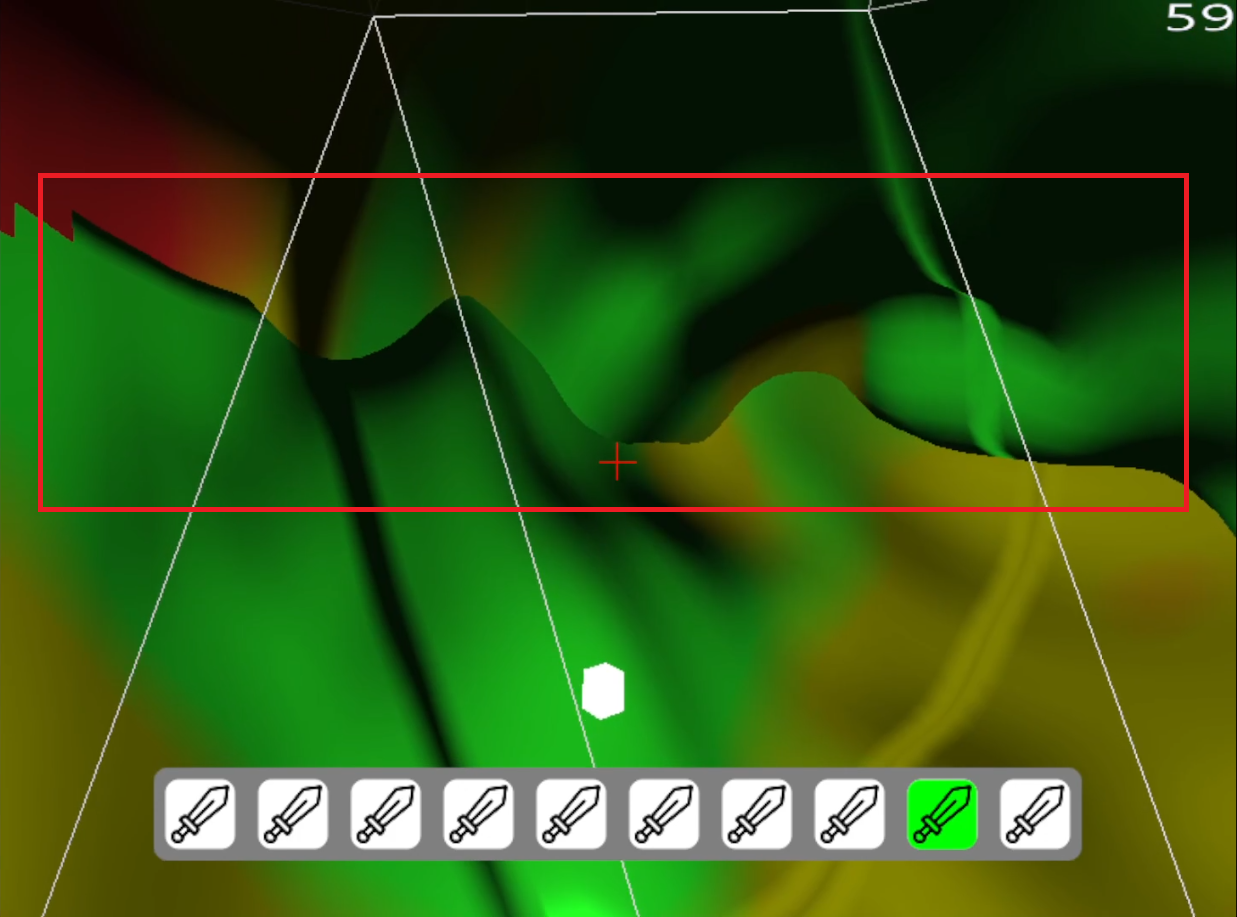
\includegraphics[width=0.6\textwidth]{chapters/problems/resources/no-terrain-stiching.png}
    \caption{Discontinuity between two regions in spherical space}
    \label{fig:no-terrain-stiching}
\end{figure}

Our solution was to modify the values of the scalar field for each region such that they combine the original scalar field $S$ (as generated by the noise function) with a \textit{boundary value} $b$ (the same for both regions).
The resultant scalar field, $S_{\mathrm{avg}}$ is defined as
\begin{equation*}
    S_{\mathrm{avg}}(x, y, z) = \mathrm{StepUp}(d, R) \cdot b(y) + \mathrm{StepDown}(d, R) \cdot S(x, y, z),
\end{equation*}
where $d$ is the distance of the point $(x, y, z)$ from the given region's center, $R$ is the region's radius (around $\pi / 2$), and the $\mathrm{StepDown}$ amd $\mathrm{StepUp}$ functions are defined as follows:
\begin{equation*}
    \mathrm{StepUp}(d, R) = \frac{1}{2} (\tanh(a (d - k R)) + 1),
\end{equation*}
\begin{equation*}
    \mathrm{StepDown}(d, R) = \frac{1}{2} (-\tanh(a (d - k R)) + 1).
\end{equation*}
The parameter $k$ describes at what distance from the region's center (relative to $R$) the boundary value starts to dominate and the $a$ parameter describes how aggressive the transition is.
Plots of the functions can be seen in \autoref{fig:step-functions}.
\autoref{fig:stiched-spheres} depicts the result of applying the aforementioned functions (the red line shows the approximate location of the boundary between regions).

\begin{figure*}[h]
    \centering
    \begin{subfigure}[b]{0.475\textwidth}
        \centering
        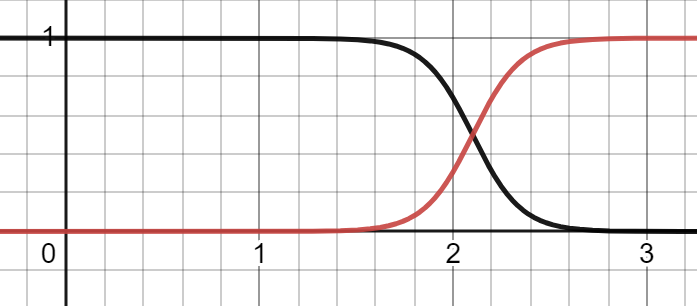
\includegraphics[width=\textwidth]{chapters/problems/resources/step-functions.png}
        \caption[]%
        {{\small $\mathrm{StepUp}$ (red) and $\mathrm{StepDown}$ (black) functions}}
        \label{fig:step-functions}
    \end{subfigure}
    \hfill
    \begin{subfigure}[b]{0.475\textwidth}
        \centering
        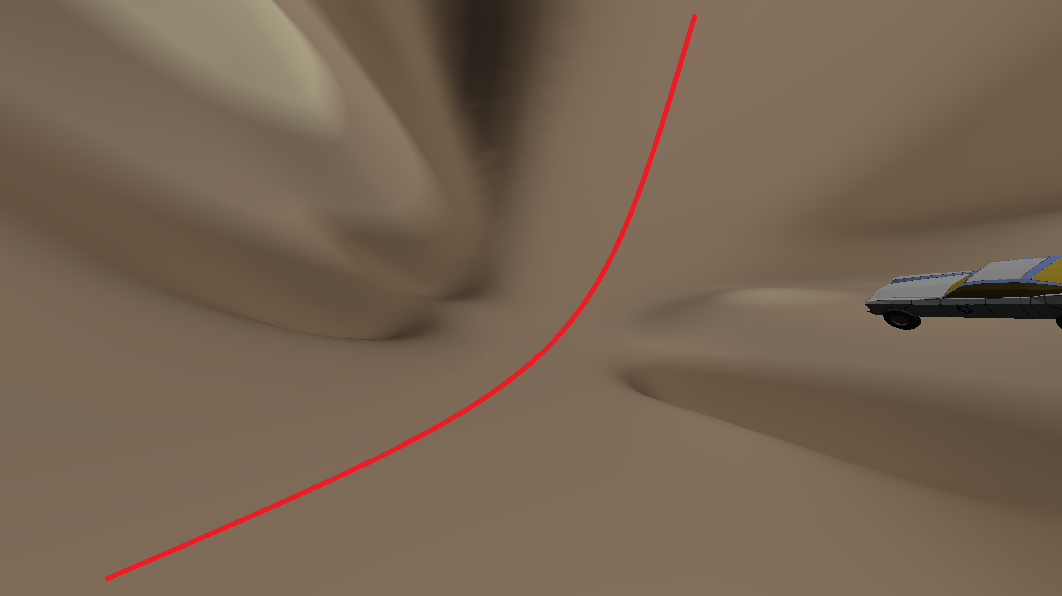
\includegraphics[width=\textwidth]{chapters/problems/resources/boundary-flat.png}
        \caption[]%
        {{\small The effect of applying the step functions}}
        \label{fig:stiched-spheres}
    \end{subfigure}
    \caption[]
    {\small Smooth transition between regions in spherical space}
    \label{fig:stiching-spheres}
\end{figure*}
In our implementation, we use $a = 0.5$ and $k = 0.75$.
The boundary value depends only on the $y$ coordinate and is simply given by $b(y) = y$ which means that the terrain generated based on this function is flat.

The last modification to the terrain generation system has to do with the average elevation of the terrain.
It turns out that points located too far from the camera are not rendered correctly\footnote{The problem is probably related to the projection matrix but we didn't investigate this further.}.
To solve this problem, the terrain is artificially elevated and mining below a certain depth is disallowed.